\section{Correlation Analysis}

\hfill \break
Their positive relation trip duration (in Seconds log-Transformed) with pickup longitude, dropoff longitude and passenger count. Figure \ref{fig:crr}

\hfill \break
There negative relation trip duration (in Seconds log-Transformed) with pickup latitude and dropoff latitude. Figure \ref{fig:crr}

\hfill \break
\textbf{Their strong positive relation trip duration (in Seconds log-Transformed) with distance}. Figure \ref{fig:crr2}

\hfill \break
Their negative relation trip duration (in Seconds log-Transformed) with speed km/h. Figure \ref{fig:crr2}

\hfill \break
\textbf{Conclusion we have a pretty good relationship between the distance features and trip duration so we can use it in modeling}. Figure \ref{fig:crr2}


\begin{figure}[ht]
\centering
    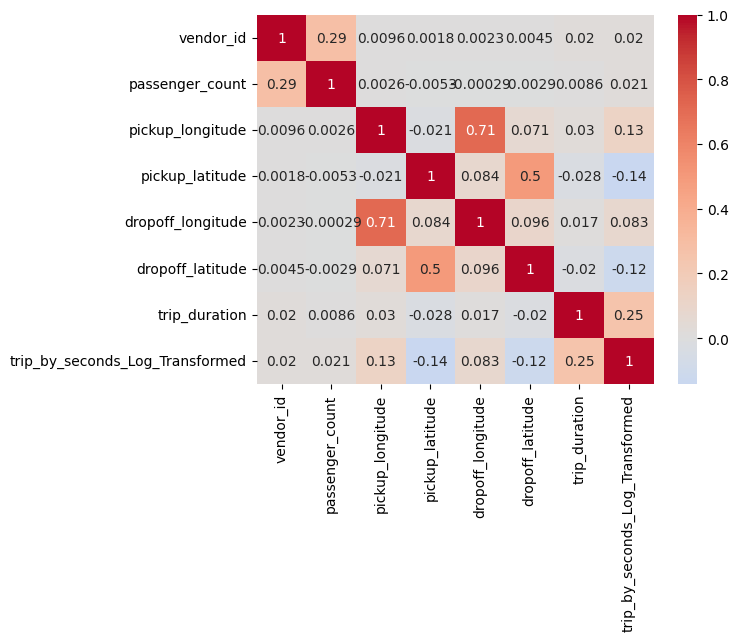
\includegraphics[width=1\linewidth]{crr.png}
    \caption{\label{fig:crr} Correlation Analysis}
\end{figure}

\hfill \break
\begin{figure}[ht]
\centering
    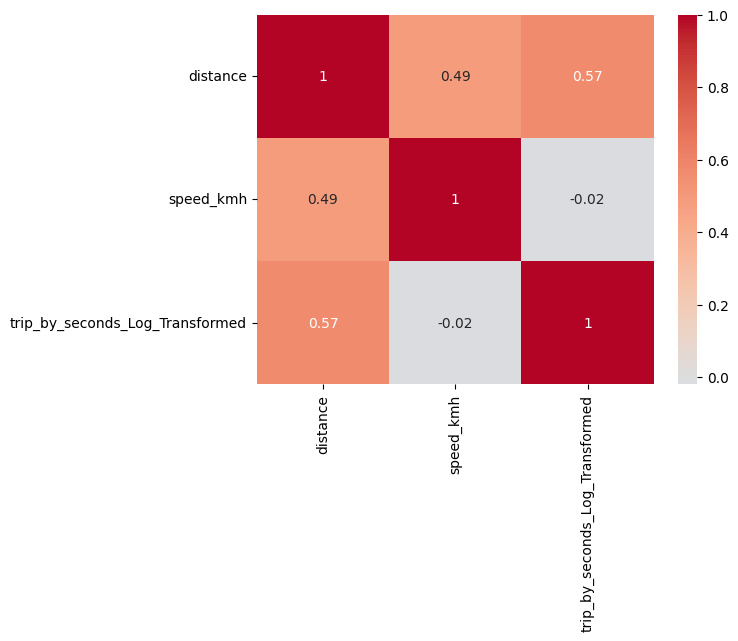
\includegraphics[width=1\linewidth]{crr2.png}
    \caption{\label{fig:crr2} Correlation Analysis}
\end{figure}

\begin{figure}
    \centering
    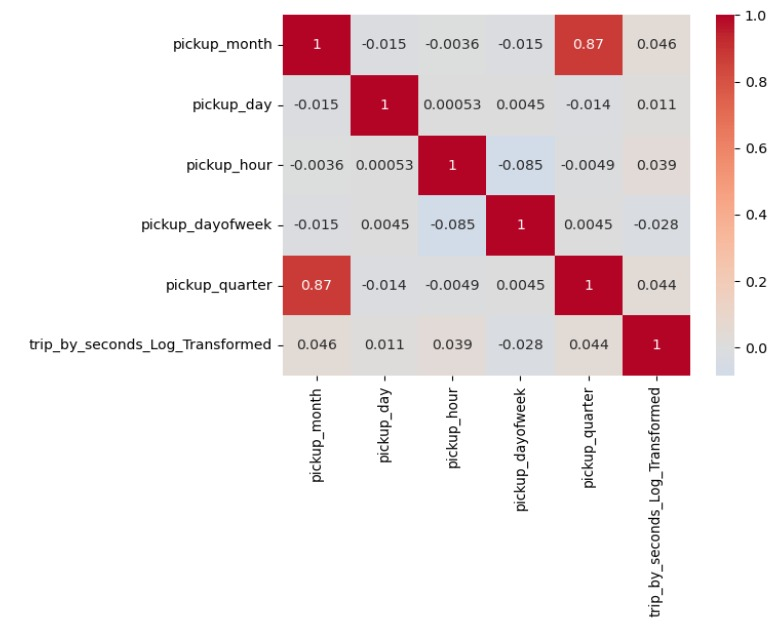
\includegraphics[width=1\linewidth]{corr3.png}
    \caption{Correlation Analysis}
    \label{fig:crr3}
\end{figure}

